%
% File colacl06.tex
%
% Contact: rlolivia@cityu.edu.hk

\documentclass[11pt]{article}
\usepackage{colacl06}
\usepackage{times}
\usepackage{url}
\usepackage{stfloats}
\usepackage{bm,array}
\usepackage{tabularx}
\usepackage{caption}
\usepackage{subfig}
\usepackage{multirow}
\usepackage{latexsym}
\usepackage{slashbox}
\usepackage{rotating}
\usepackage{amsmath}
\setlength\titlebox{6.5cm}    % Expanding the titlebox

\title{Plagiarism Detection using Text Mining}

\author{First Author\\
  Affiliation / Address line 1\\
  Affiliation / Address line 2\\
  Affiliation / Address line 3\\
  {\tt email@domain}  \And
  Second Author\\
  Affiliation / Address line 1\\
  Affiliation / Address line 2\\
  Affiliation / Address line 3\\
  {\tt email@domain}}

\date{}

\begin{document}
\maketitle
\begin{abstract}
  Plagiarism has been an increasing concern in various fields, in particular, academia. The availability of enormous amount of resources on the web and the increasing usage of electronic media are the major causes for increase in plagiarism. A significant contribution of the paper is to use Natural Language Processing techniques to integrate linguistic and background knowledge from resources such as WordNet and Wikipedia into the plagiarism detection process. The process is computationally intensive, and our second contribution is to tailor traditional text mining techniques to speed up detection. Experiments have been performed on a corpus of short answers containing different levels of plagiarism. Results show the advantage of considering semantics in plagiarism detection over standard methods based on naive string matching and n-grams. Finally, {\em  winnowing}, a fingerprinting algorithm, is shown to be effective in improving the efficiency of both the storage and detection process.
\end{abstract}

\section{Introduction}\label{1}

Plagiarism is an act of using content or ideas of other people and presenting them as one's own work without proper acknowledgement of the original source(s). It is generally prominent in areas such as academics, scientific research and journalism. There are different forms of plagiarism depending on the way in which the content of the source(s) is extracted, modified and presented in the actual work.

Plagiarism detection is an important process for maintaining integrity and fostering ethical research values among students. Innumerable resources have been made freely available on the internet for general public which could serve as sources of plagiarism. This has created the need for automation of detection process which needs to be robust and accurate simultaneously. In this paper, we constrain our focus to plagiarism detection of text documents in English.

In the recent past, some online plagiarism detection tools have been developed and made available commercially as well as for free. Majority of academic institutions use popular online tools such as Turnitin or PlagScan which use techniques that can detect cases of verbatim plagiarism with high efficiency and accuracy. Their basic idea is to compute and find sequences of matching keywords of length greater than some threshold. Other techniques involved include fingerprinting, matching n-grams, (generally, bigrams and trigrams) and vector space models (bag of words). These approaches are based on the characteristic distribution of words in a language, also known as Zipfian distribution~\cite{manning:99}. In other words, as the size of n-gram increases, its frequency in independently written texts decreases.

Existing approaches generally do not consider the meanings or senses of different words and concepts. As a result, they fail in comparing synonyms or similar words, different syntactic forms of a word, and concepts which require some background knowledge of the subject. Hence, these approaches are ineffective in detecting cases involving paraphrasing, changes in order or words, syntactic changes and plagiarism of ideas. These instances need more involved semantic relatedness measures to detect them and distinguish the various levels of plagiarism.

In this paper, we attempt to overcome these limitations by integrating knowledge from sources like Wikipedia and lexical resources like WordNet into the detection process. The concept of clustering similar words and concepts is applied to generalise them and therefore, recognize pieces of paraphrased text. Text mining techniques like fingerprinting and winnowing are used to identify plagiarism cases and distinguish the different levels of plagiarism. Other NLP concepts like Word Sense Disambiguation (WSD), Part of Speech (POS) tagging and parsing are also used to identify the appropriate senses and extract different words and concepts from the text for comparison. Features like sorted n-grams and matching subsequences of texts are derived and used to classify instances into different classes of plagiarism using Naive Bayes classifier.

The paper is organized into different sections as follows. Section \ref{2} gives a brief account of the related work. Section \ref{3} provides a detailed description of our approach with an illustration. Experimental setup and results are presented in Section \ref{4}. Section \ref{5} analyzes the advantages and shortcomings of the ideas proposed. Finally, we conclude our work by summarizing our main contributions.

\section{Related Work}\label{2}
 Recently, Meuschke and Gipp~\shortcite{meu:13} discussed the state-of-the-art methods in plagiarism detection. Plagiarism detection is generally categorized into two major categories, namely, intrinsic and extrinsic plagiarism detection. Intrinsic plagiarism detection is the process of detecting instances without any reference corpus containing potential sources. It involves modelling the writing style of the author using character n-gram profiles and measuring its deviation within the suspicious document~\cite{sta:09}.

Extrinsic plagiarism detection refers to the process in which suspicious documents are compared against a corpus containing a set of potential source documents. It has been the major focus of research in the past. One of the earliest attempts was made by Lyon et al.~\shortcite{lyon:04} in the form of Ferret electronic plagiarism detection system. Their implementation was based on matching trigrams between the source and suspicious documents which performed well, however, it failed to handle cases where there were simple additions and deletions of words.  Further, Nahnsen et al.~\shortcite{nah:05} extended this idea by using lexical resources like the WordNet and applied WSD to keywords. They computed cosine similarity between pairs of vectors of lexical n-grams and  tf-idf weighted keywords. Lexical chains were extracted using an algorithm proposed by Silber and McCoy~\shortcite{sil:02}. Although there was some considerable improvement, the same drawback holds in this approach too. Also, both the processes of WSD and lexical chain extraction could themselves be inaccurate as they are complex and have their own limitations.

Later, Clough and Stevenson~\shortcite{clough:11} designed a corpus of short answers (in 2009) comprising instances pertaining to different levels of plagiarism and experimented on them. Features like different sized n-grams and longest common subsequence (LCS) were used to classify the suspicious documents. They achieved a high accuracy in binary classification using Naive Bayes classifier but their approach would not account for basic cases like synonyms substitution as there is no semantic interpretation of text.

Chong et al.~\shortcite{chong:10} demonstrated the importance of NLP techniques in detecting plagiarism. Preprocessing comprised vital steps like sentence segmentation, stemming and POS tagging. In addition to the features used by Clough and Stevenson~\shortcite{clough:11}, language model probability (perplexity) and dependency relations matching were used in their experiments on the same corpus of short answers. Results displayed significant improvement over the state-of-the-art methods and the Ferret baseline. Their work was further extended by Chong and Specia~\shortcite{chong:11} through lexical generalisation. They experimented on a subset of PAN'10 corpus and showed their approach yielded better results than standard n-gram techniques. Their idea was to expand text by replacing each word with synonymous words in all the synsets of the same word. However, they do not consider potential matching subsequences which do not have any common n-grams. Moreover, in many instances, paraphrasing might involve substituting words which are related to each other but not necessarily synonyms.

Ceska and Fox~\shortcite{ceska:11} later investigated the effect of preprocessing techniques on a corpus containing Czech documents. Processes like recognizing synonyms, generalising words based on WordNet, and replacing numbers with dummy values have helped improve accuracy. However, they concluded that not all the preprocessing steps proved useful and that some only helped in reducing execution time. Results have not been satisfactory as they do not consider the order in which the matches occur and could also be due to an inaccurate process of generalising words.

Nawab et al.~\shortcite{nawab:12} suggested a similar method which detects text reuse by creating modified and weighted n-grams from the original n-grams. They performed their experiments on the METER corpus~\cite{gai:01} and reported improvement compared to the approaches existed at that time. Modified n-grams are created by deleting a single word or by substituting synonyms for all possible senses of a word in the original n-grams. This approach might handle operations like deletions or insertions of words but is still limited due to other drawbacks mentioned in the case of Chong et al.~\shortcite{chong:10} and Chong~\shortcite{chong:11}.

Recently, Kumar~\shortcite{kumar:14} proposed an advanced graph based approach for handling word reordering and paraphrasing in text. His experiments on PAN'12 corpus and the corpus created by Clough and Stevenson~\shortcite{clough:11} resulted in a better performance over the existing methods. It involves creation of a semantic network (terms as nodes) using a sliding window for creating links weighted using co-occurrence frequency and normalised Pointwise Mutual Information of the terms. Further, the concept of minimum weighted bipartite clique is used to identify the plagiarised text patterns in the source and suspicious texts. Advanced NLP techniques involving semantics and background knowledge of the text have not been thoroughly explored. This paper attempts to fill this gap. We also address efficiency overheads that are a downside of the more sophisticated matching process.

\section{Our Approach}\label{3}
We implement our method in three stages. Initially, we apply the standard preprocessing techniques to remove noise and convert the text into a uniform format, making it easier for analysis. Further, we use WordNet and Wikipedia based semantic relatedness measures to cluster similar pieces of text together. We perform fingerprinting in order to represent each document uniquely. Eventually, the document fingerprint is used to extract n-grams and compute LCS which are used as features to establish similarity between document pairs. The complete process is illustrated with an example shown in Table \ref{ex} which is adapted from Indiana University's website (\url{http://www.indiana.edu/~wts/pamphlets/plagiarism.shtml}).

\begin{table}[h]
\footnotesize
\begin{tabularx}{\columnwidth}{|X|}
\hline
\textbf{Original:} The rise of industry, the growth of cities, and the expansion of the population were the three great developments of late nineteenth century American history. As new, larger, steam-powered factories became a feature of the American landscape in the East, they transformed farm hands into industrial laborers, and provided jobs for a rising tide of immigrants. With industry came urbanization the growth of large cities (like Fall River, Massachusetts, where the Bordens lived) which became the centers of production as well as of commerce and trade.\\
\hline
\textbf{Plagiarised:} The increase of industry, the growth of cities, and the explosion of the population were three large factors of nineteenth century America. As steam-driven companies became more visible in the eastern part of the country, they changed farm hands into factory workers and provided jobs for the large wave of immigrants. With industry came the growth of large cities like Fall River where the Bordens lived which turned into centers of commerce and trade as well as production.
\\
\hline
\end{tabularx}
\caption{Example for plagiarism}
 \label{ex}
\end{table}

\subsection{Preprocessing}
 We use the Stanford CoreNLP package (version 3.3.1) publicly available at the Stanford NLP Group \footnote{\url{http://www-nlp.stanford.edu/}} which provides a set of natural language processing tools for analysing English text. As a part of preprocessing, we split the text into individual sentences and parse them using the Stanford Parser. We extract concepts, nouns and common phrases by applying simple heuristics like considering phrases starting with upper case letters. These different words, nouns and concepts form the set of tokens. We replace numbers with a common symbol and convert all other letters to lowercase for uniform comparisons. Extra characters like punctuation marks are removed. We also remove all stopwords by maintaining a dictionary of such words to ensure these frequently occurring words do not affect comparison. We use the Stanford POS tagger to assign the Penn Treebank part-of-speech tags to all the words. These tags are appropriately mapped to the POS tags used in various synsets in WordNet. Individual words are then lemmatized to their basic forms or {\em  lemmas} for comparing inflected forms of the same word.

\paragraph{Word Sense Disambiguation} In this experiment, we avoid the actual WSD process which is complex because the state-of-the-art methods have not attained satisfactory levels of accuracy. Instead, we prune the set of different possible senses of a given word by comparing the POS tags of its different possible synsets with the tag assigned by the Stanford tagger. 

WSD is important for proper clustering of words which are synonymous or related to each other. A word might be synonymous or highly similar to two different words with respect to two different senses of the same original word. For example, the word ``light" could be related to both ``glow" and ``weight" in two different senses. Clustering based on similarities estimated using all possible synsets of a word would result in unrelated words like ``glow" and ``weight" to belong to the same cluster making it incoherent.

\subsection{Clustering}
Preprocessed tokens are clustered using semantic relatedness measures. Semantic relatedness is a similarity metric
between two terms or documents based on their meaning and information content. Generally, semantic relatedness between terms is estimated based on their
positions in a taxonomy using path based similarity measures.

\subsubsection*{WordNet based similarity}
The Natural Language Tool Kit (\url{http://www.nltk.org/})  provides implementations of several algorithms for measuring semantic relatedness between words using WordNet~\cite{mih:06}. Some examples include Resnik similarity~\cite{res:95}, Wu-Palmer similarity~\cite{wu:94} and Leacock Chodorow similarity~\cite{lea:98}.

In our experiments, we use the Wu-Palmer similarity for estimating semantic similarity between words. It computes similarity based on the depth of the two synset nodes in the WordNet taxonomy and the depth of their Least Common Subsumer (LCS) node. Wu-Palmer similarity between two synsets, sub 1 and sub 2, is estimated using the Equation  \ref{wup}. Its range is (0,1].
\begin{equation}   \label{wup}\small
{wup\_similarity} = \frac{ 2* \text{depth(LCS)}}{\text{depth(sub 1)} + \text{depth(sub 2)}}
\end{equation}  
Semantic relatedness between two words is estimated as the maximum similarity score among the {\em  wup\_similarity} scores obtained for every possible synset pair formed by taking one synset from the set of possible senses for each word after pruning.

\subsubsection*{Wikipedia based similarity}
Explicit Semantic Analysis (ESA)~\cite{gab:07} is a method used to represent the meaning of text as a weighted vector of concepts in a high dimensional space of concepts derived from a corpus (Wikipedia in specific). Semantic relatedness between two texts is estimated using standard similarity metrics used for comparing vectors (eg. cosine similarity).

ESA provides us the background knowledge that is required to compare text, specific to a particular concept or field, which cannot be compared in a meaningful way using lexical resources like WordNet. We use ESA to compute similarities of remaining tokens comprising concepts, nouns and words which are not present in the WordNet. We use a publicly available implementation of an algorithm proposed by Gabrilovich and Markovitch~\shortcite{gab:07} to perform ESA. For example, let us consider a toy Wikipedia having only four articles. The words are represented as vectors in a 4-dimensional concept space derived from these articles. Let c$_{1}$, c$_{2}$, c$_{3}$ and c$_{4}$ be the four concepts derived. Table \ref{esa} shows the computation of similarity between two words, w$_{1}$ and w$_{2}$, using the algorithm.
%``frequentist" and ``bayesian" are of length 19 and 135 respectively. The cosine similarity value obtained is 0.475.

\newcolumntype{C}{>{\centering\arraybackslash}p{2em}}
\begin{table}[h]
\small
    \begin{center}
     \begin{tabular}{|C|C|C|C|C|}
     	\hline
        & c$_{1}$ & c$_{2}$ & c$_{3}$ & c$_{4}$\\
      \hline
       w$_{1}$ & 3 & 1 & 2 & 4\\ 
      \hline
       w$_{2}$ & 2 & 4 & 0 & 3 \\ 
      \hline 
      \multicolumn{5}{|c|}{Cosine similarity = ${\frac{22}{\sqrt{30*29}} = 0.75}$}\\
      \hline
      \end{tabular}
    \end{center}
    \caption{Example for ESA of two words}
	  \label{esa}
 \end{table}
 
\subsubsection*{Agglomerative Hierarchical Clustering}
Agglomerative hierarchical clustering is a bottom up strategy to build large clusters incrementally~\cite{tan:06}. We follow the MIN strategy to merge intermediate clusters repeatedly. In this strategy, we merge two intermediate clusters having the most similar pair of words. Group average strategy could also be used but it might result in rigid clusters containing only synonyms, unlike the MIN strategy which is more permissive for grouping related words.

In our method, we use the semantic relatedness measure computed using WordNet and Wikipedia for clustering tokens. During clustering, both the WordNet and ESA based similarities are compared to their respective thresholds independently. After clustering, each cluster is assigned a random integer which is its unique identity.
 
 Table \ref{fp} shows the representation of the example texts using cluster identities after clustering the words with a similarity threshold of 0.85 for WordNet based similarities. For a recall-centric system, low threshold is chosen as it helps in generalising words which results in increase of similarities and hence, higher recall. For a precision-centric system, the threshold is chosen close to 1.0.
 
\begin{table}[h]
\footnotesize
\begin{tabularx}{\columnwidth}{|X|X|}
\hline \multicolumn{1}{|c|}{ \textbf{Original}} &  \multicolumn{1}{c|}{\textbf{Plagiarised}} \\
\hline
4 7 4 9 4 7 12 3 4 13 14 15 16 17 18 3 19 10 2 1 7 16 20 21 22 7 7 23 7 10 7 1 24 25 7 1 26 4 3 9 27 4 28 29 30 31 1 9 7 32 7 7
&
4 7 4 9 4 7 12 3 7 14 15 9 19 10 33 1 34 35 7 9 1 7 7 2 36 10 7 3 4 25 7 1 4 3 9 27 4 28 30 31 1 9 7 7 32 7\\
\hline
\end{tabularx}
\caption{Representation using cluster identities}
 \label{fp}
\end{table}

\subsection{Comparison Methodology}
The following procedure is followed to compare the preprocessed texts using the results obtained from clustering.

\subsubsection*{Fingerprinting} 
Fingerprinting is a widely used method for extrinsic plagiarism detection. Document fingerprinting is an algorithm to represent a document uniquely with a sequence of hashes for comparison and other analysis purposes. It helps in avoiding storage and comparison of large pieces of text and improves the execution time.

We use the Rabin-Karp Hash function formulated by Karp and Rabin~\shortcite{karp:87} for hashing n-grams. It is a recursive hash function used to compute the hash value of a sequence of elements (generally, n-grams) for efficient string matching. The function enables calculation of hash value of $(i+1)^{st}$ n-gram from the hash value of $i^{th}$ n-gram. Let $w_{1}w_{2}..w_{n}$ be an n-gram of words where each $w_{i}$ represents the unique identity of a word. The hash value of the n-gram $f(w_{1}w_{2}..w_{n})$ is defined in Equation \ref{eq}.
\begin{equation}   \label{eq}
\small
f(w_{1}w_{2}..w_{n}) = w_{1}b^{n-1} + w_{2}b^{n-2}... + w_{n-1}b + w_{n}
\end{equation}  
Hash value of next overlapping or $(i+1)^{st}$ n-gram is computed using the identity in Equation  \ref{id}.
\begin{equation}   \label{id}
\small
f(w_{2}w_{3}..w_{n+1}) = f(w_{1}w_{2}..w_{n}) - bw_{1}b^{n-1} + w_{n+1}
\end{equation}  
Base {\em  b} is generally chosen to be a prime number to ensure uniform distribution and prevent collision of hash values. In our experiments, we consider k-grams of tokens in which tokens are represented by their unique identities. k-grams help in detecting reuse of text irrespective of the order of paragraphs or sentences within the documents.

\paragraph{Sorting k-grams}  k-grams are also sorted based on the numerical values of their constituent token identities. Sorting k-grams helps in detecting re-ordering of tokens within the k-gram as observed for the last two trigram hashes in Table \ref{hash}. Unsorted k-grams common to both the fingerprints would still be matched, even after sorting.

Table \ref{hash} shows the fingerprints of the example texts after hashing trigrams. Here, {\em k} = 3 and {\em b} = 31. For example, the hash value of the first trigram in Table \ref{fp}, ``4, 7, 4", after sorting is computed as $f(4, 4, 7) = 4*31^{2} + 4*31 + 7 = 3975$.

\begin{table}[h]
\footnotesize
\begin{tabularx}{\columnwidth}{|X|}
\hline
\textbf{Original:} \textbf{3975}, \textbf{4070}, \textbf{3977}, \textbf{4070}, \textbf{4073}, \textbf{3112}, 3019, 3020, 4261, 12942, 13935, 14928, 15921, 3428, 3460, 3212, 2251, 1033, 1030, 1194, 7243, 16017, 19893, 7400, 6966, 6967, 6967, 7060, 6954, 1188, 1202, 1730, 7496, \textbf{1203}, 1204, 1111, 3033, \textbf{3016}, 3189, \textbf{4150}, \textbf{4709}, 4741, 27837, 28830, \textbf{1922}, \textbf{1271}, \textbf{1187}, 7038, \textbf{6976}, \textbf{6976}\\
\hline
\textbf{Plagiarised:} \textbf{3975}, \textbf{4070}, \textbf{3977}, \textbf{4070}, \textbf{4073}, \textbf{3112}, 3112, 3114, 7176, 9098, 9133, 8978, 10232, 1304, 2018, 2050, 7816, 7041, 1187, 1187, 1185, 2146, 2175, 2268, 7073, 3110, 3014, 3032, 4086,\textbf{ 1203}, 1092, 1058, \textbf{3016}, 3189, \textbf{4150},\textbf{ 4709}, 4742, 27869, \textbf{1922},\textbf{ 1271}, \textbf{1187}, 6953, \textbf{6976}, \textbf{6976}
\\
\hline
\end{tabularx}
\caption{Fingerprints after hashing sorted trigrams}
 \label{hash}
\end{table}

\subsubsection*{Similarity features}
We extract relevant features from the fingerprints containing k-gram hashes for classification.

\paragraph{Containment measure}  Containment measure, as defined by Clough and Stevenson~\shortcite{clough:11} is used to establish similarity between documents based on their common k-grams. Let A be the suspicious document and B be the source document. S(A,k) and S(B,k) represent the set of k-grams in the suspicious and source documents respectively. The containment measure is defined  as {\small $C_{k}(A,B) =  \frac{{\displaystyle|S(A, k) \cap S(B, k)|}}{ {\displaystyle|S(A, k)|}}$}. It is normalised by the number of k-grams in the suspicious document which helps in comparing suspicious documents with varying lengths. In our corpus, the source documents are always larger in size than the corresponding suspicious documents.
 
\paragraph{Longest Common Subsequence (LCS)} We compute the LCS between source and suspicious document fingerprints. LCS matches sequences of tokens reused in the same order which might not be a part of any matching k-gram. For example, the two sequences, ``a b d e" and ``a b \textbf{c} d e", have four common elements in order but no matching trigrams. We use the normalised LCS measure defined as {\small ${LCS}_{norm} = \frac{\displaystyle {LCS(A, B)}}{\displaystyle {Length(A)}}$}.  

\subsubsection*{Winnowing} 
Winnowing is an algorithm for selecting particular hashes from a sequence of  hashes of k-grams~\cite{sch:03}. Here, we consider k-grams of tokens. Fingerprinting algorithms generally satisfy two important properties for matching substrings between documents. First, they provide a {\em  guarantee threshold, t,} such that any matching substring containing atleast {\em  t} tokens would necessarily contain a matching k-gram hash in both the fingerprints.
 Second, they have a {\em  noise threshold, k ($\geq t$),} below which n-grams ($n < k$) are not matched considering them as noise. Higher values of {\em  k} minimize the probability of coincidental or irrelevant matches. However, very large values of {\em  k} might not detect reordering, deletions or insertions within substrings of length less than {\em  k} tokens. Therefore, the choice of {\em  k } value is critical for comparison.
	
	In this algorithm, the minimum hash value is selected in every window of size, {\em  w}, containing {\em  w} k-gram hashes. If there is more than one hash with same value as the minimum, we choose the rightmost occurrence. The selected set of hashes form the winnowed fingerprint of the document. We choose the minimum value to ensure that there is at least one hash value from every window and to simultaneously reduce the length of the fingerprint by a significant factor. For a chosen pair of values, {\em  k} and {\em  t}, window size, $w  = t - k + 1$.
	
	 For example, let us say, given a fingerprint containing a sequence of hashes of trigrams ({\em k = 3}) of tokens , we are required to identify every matching sequence of tokens of length, $t \geq 6$ (essentially, 6-grams and above). In a 6-gram, there are 4 overlapping trigrams. Hence, by choosing a window of size 4 (= 6 - 3 + 1), we select at least one trigram hash  from that window according to winnowing. In the sample text, (4,7,4,9,4,7) is a matching 6-gram. The 4 trigram (sorted) hashes corresponding to it are 3975, 4070, 3977 and 4070. If we choose a window size of {\em w = 4}, then at least one (here, 3975) of these will be present in the fingerprint to represent the 6-gram match. 
	 
	 Winnowing not only guarantees the matching of sequences of length at least {\em t}, but it can also match sequences of length $<$ t (and $\geq k$) with some  probability when the minimum hash value in a window is part of a matching n-gram ($k \leq n < t$).  This kind of matching cannot be achieved by directly matching t-grams. In the above example, if only (4,7,4,9) was common, it would still be identified because the minimum hash (= 3975) is of the trigram (4,7,4) which is a part of this matching 4-gram.

	Expected length of the document after winnowing is equal to $\frac{2}{w+1}$ times its original length. This is because only two out of the ({\em  w} + 1) possible cases contribute a new hash to the fingerprint in case of a new window. The cases are: 1) Previous minimum hash value does not occur in the new window. 2) New hash added is the new minimum hash value.
 
 In the sample case under consideration, the fingerprints obtained after winnowing using a window of a size w = 3 are shown in Table \ref{win}. The lengths of the original and plagiarised texts are reduced from 50 to 33 and 44 to 29 respectively (slightly greater than the expected lengths). The containment measure computed without winnowing, C$_{k}=0.340$ (=$\frac{15}{44}$) is almost equal to the value after winnowing, C$_{k_{win}}=0.345$ (=$\frac{10}{29}$).

\begin{table}[h]
\footnotesize
\begin{tabularx}{\columnwidth}{|X|}
\hline
\textbf{Original:} \textbf{3975}, \textbf{3977}, \textbf{3112}, 3019, 3020, 4261, 12942, 13935, 3428, 3212, 2251, 1033, 1030, 1194, 7243, 7400, 6966, 6967, 6967, 6954, 1188, 1202, \textbf{1203}, 1204, 1111, \textbf{3016}, 3189, \textbf{4150}, \textbf{4709}, 4741,\textbf{ 1922}, \textbf{1271}, \textbf{1187}, 6976\\
\hline
\textbf{Plagiarised:} \textbf{3975}, \textbf{3977}, \textbf{3112}, 3112, 3114, 7176, 8978, 1304, 2018, 2050, 1187, 1187, 1185, 2146, 2175, 2268, 3014,\textbf{ 1203}, 1092, 1058, \textbf{3016}, 3189, \textbf{4150}, \textbf{4709}, \textbf{1922}, \textbf{1271}, \textbf{1187}, 6953
\\
\hline
\end{tabularx}
\caption{Fingerprints obtained after winnowing}
 \label{win}
\end{table}

\subsubsection*{Choice of Parameters}  For measuring containment measure, the choice of k is generally 2 or 3. Trigrams result in a higher precision without compromising on recall as compared to bigrams which might contain irrelevant or noisy matches. For higher values of k, the accuracy values would be low due to lower recall. Choice of window size {\em  w} has a similar effect as {\em k} as it determines the minimum size of n-gram to detect. In case of similarity, threshold values $\le$ 1 magnify the similarities as the words are generalized. However, recall or accuracy might not necessarily improve with  very less threshold values. This is because the magnified similarities could cause the machine learning algorithm to learn a higher similarity threshold to detect plagiarised cases and might fail to detect slightly plagiarised cases whose similarity values are unaffected by word generalization. This effect has been observed in the experiments we performed.

\section{Empirical Evaluation}\label{4}
We evaluate our approach by experimenting on the corpus of short answers.
\subsection{Corpus}
In our experiments, we use the corpus created by Clough and Stevenson (in 2009). The corpus was manually developed using five Wikipedia articles as the source documents. Corpus contains a total of 95 suspicious documents with different levels of plagiarism. 19 students were asked to write their responses to 5 questions, each question based on a different article in the sources. Documents were classified into four classes based on pre-defined guidelines given to the students.
 \begin{enumerate}
 \itemsep0em
 \item Near copy: Text was simply copied from the original text without any changes.
 \item Light revision: Copying by substituting words and phrases with synonyms, addition or deletion of some phrases and changes in grammatical structure. Order of the sentences was preserved.
 \item Heavy revision: Rephrasing and restructuring  sentences using their own words. It also involved splitting and combining sentences.
 \item Non plagiarism: Answers written based on student's own knowledge and learning from sources like text book chapters and notes without access to the original articles.
 \end{enumerate}
 
  Each suspicious document was about 200-300 words in length. There were 38 non-plagiarised documents and 19 in each of the other three categories. Although there are other corpora like the METER corpus~\cite{gai:01} or the standard PAN corpus, this particular corpus was chosen as it is well annotated and contained different levels of plagiarism. Moreover, it reflects a more realistic situation compared to other corpora where plagiarism is artificially introduced through automated operations like copying, inserting or merging content from documents that are selected randomly. Such corpora would not reflect the advantages of applying deep NLP techniques.


\begin{table*}[t]
\small
  \begin{center}
  \begin{tabular}{|c|c|c|c|c|c|c|c|c|c|}
	\hline
    \multirow{2}{*}{{\em  Class}} & \multicolumn{3}{ c }{{\em  Precision}} & \multicolumn{3}{ |c| }{{\em  Recall}} & \multicolumn{3}{c| }{{\em  F-measure}} \\
    \cline{2-10}
     & Ferret & Chong & \textbf{Ours }& Ferret & Chong & \textbf{Ours} & Ferret & Chong & \textbf{Ours} \\
    \hline
    {Non} & 0.884 & 0.881 & 0.905 & 1.0 & 0.974& 1.0 & 0.938  & 0.925& 0.95 \\
    \hline 
    Cut & 0.615 & 0.667 & 0.733& 0.421 & 0.526 & 0.579& 0.5 & 0.588 & 0.647 \\ 
    \hline 
    Heavy & 0.419 & 0.55 & 0.522 & 0.684 & 0.579 & 0.632 & 0.52 & 0.564 & 0.571 \\ 
    \hline 
    Light & 0.5 & 0.5 & 0.6 & 0.211 & 0.474 & 0.474 & 0.296 & 0.486 & 0.529 \\ 
    \hline 
    Weighted Average &  0.66 & 0.696 & \textbf{0.733} & 0.663  & 0.705 & \textbf{0.737} & 0.639 & 0.698 & \textbf{0.73} \\ 
    \hline 
    Macro Average & 0.605 & 0.65 & \textbf{0.69} & 0.579  & 0.638 & \textbf{0.671} & 0.592  & 0.644 & \textbf{0.68} \\ 
    \hline 
 \end{tabular}
 \end{center}
 \caption{Precision, Recall and F-measure values obtained for each class in multiclass classification task by the Ferret, model designed by Chong et al.~\shortcite{chong:10} and our model with Naive Bayes Classifier}
 \label{t1}
 \end{table*}
 
\subsection{Classification Task}
We perform both multiclass classification and binary classification of the suspicious documents. In binary classification, we classify the documents as either plagiarised or non-plagiarised. In multiclass classification, our goal is to classify the suspicious documents into the four categories described previously. Containment measure and LCS$_{norm}$ are used as features for the purpose of classification. 

From the graph in Figure \ref{graph}, we can observe the progression of similarity values from ``non" to ``cut" category. The ``non" plagiarised documents are well clustered and distinguished from the plagiarised ones. However, the other points are almost uniformly scattered and are not linearly dependent on the level of plagiarism indicating the difficulty in classifying them. We use these two features for classification using Naive Bayes classifier. We use the simple Naive Bayes classifier with 10-fold cross validation which is implemented in Weka~\cite{hall:09}, a machine learning software.
 
 \begin{figure}[h]
   \begin{center}
	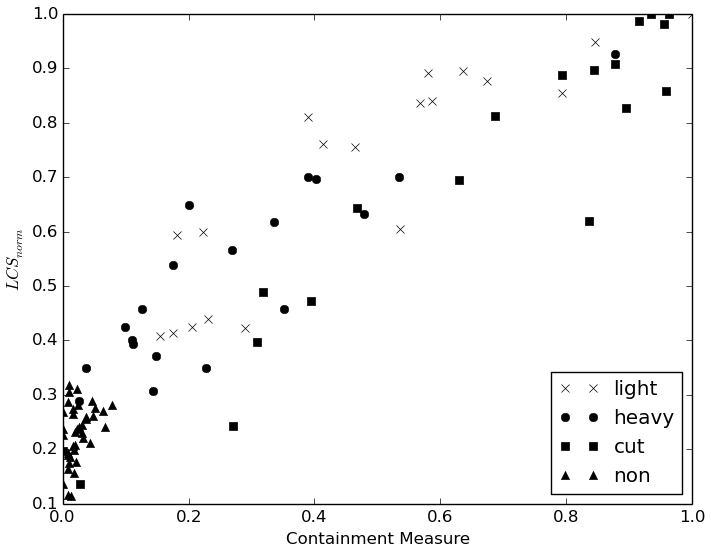
\includegraphics[width=\columnwidth]{graph2.png}
     \caption{Correlation graph between LCS$_{norm}$ and Modified Jaccard Similarity}
   \label{graph}
   \end{center}
\end{figure}

\begin{table*}[bp]
\small
    \begin{center}
     \begin{tabular}{cc|c|c|c|c|ccc|c|c|c|c|}
     \cline{3-6}\cline{10-13}
      & & \multicolumn{4}{c|}{Predicted Class - Our model}& & & & \multicolumn{4}{c|}{Predicted Class - Chong model}\\
      \cline{3-6}\cline{10-13}
      & & Non & Cut & Heavy & Light&  & & & Non & Cut & Heavy & Light\\
      \cline{1-6}\cline{8-13}
      \multicolumn{1}{ |c| }{\multirow{4}{*}{\rotatebox{90}{Original}}} & Non & \textbf{38} & 0 & 0 & 0 & &\multicolumn{1}{ |c| }{\multirow{4}{*}{\rotatebox{90}{Original}}} & Non & \textbf{38} & 0 & 0 & 0\\ 
      \cline{2-6} \cline{9-13}
      \multicolumn{1}{ |c| }{} & Cut & 2 & \textbf{11} & 4 & 2 & & \multicolumn{1}{ |c| }{} & Cut & 2 & \textbf{10} & 2 & 5\\ 
      \cline{2-6}\cline{9-13}
      \multicolumn{1}{ |c| }{} & Heavy & 2 & 1 & \textbf{12} & 4 & &  \multicolumn{1}{ |c| }{} & Heavy & 3 & 1 & \textbf{11} & 4\\ 
      \cline{2-6} \cline{9-13}
      \multicolumn{1}{ |c| }{} & Light & 0 & 3 & 7 & \textbf{9} & & \multicolumn{1}{ |c| }{} & Light & 0 & 4 & 6 & \textbf{9}\\ 
      \cline{1-6}\cline{8-13}
     \end{tabular} %
    \end{center}
    \caption{Confusion matrices obtained for our model (left) and Chong et al. ~\shortcite{chong:10} model (right)}
	  \label{t3}
 \end{table*}%
 
\subsection{Baseline Models}
We use the Ferret plagiarism detection tool and the model by proposed by Chong et al.~\shortcite{chong:10} as our baseline classifiers and compare our approach against them. Ferret uses Jaccard similarity coefficient to measure the similarity between source and suspicious documents by matching trigrams in both. Let A and B be the two documents and S(A) and S(B) represent the set of their trigrams respectively. Jaccard coefficient is defined as {\small ${J(A,B)} = \frac{{\displaystyle |S(A) \cap S(B)|}}{{\displaystyle |S(A) \cup S(B)|}}$}. Chong et al.~\shortcite{chong:10} used standard preprocessing techniques and also applied NLP concepts like language models and dependency parsing to obtain different features, in addition to containment measure and LCS$_{\text{norm}}$, for classification using Naive Bayes classifier.

%\begin{table*}[htbp]
%  \small
%  \centering
%  \subfloat[Indexing Performance]{%
%    \hspace{.5cm}%
%    \begin{tabular}{cc|c|c|c|c|}
%     \cline{3-6}
%      & & \multicolumn{4}{c|}{Predicted Class}\\
%      \cline{3-6}
%      & & Non & Cut & Heavy & Light\\
%      \cline{1-6}
%      \multicolumn{1}{ |c| }{\multirow{4}{*}{\rotatebox{90}{Original}}} & Non & \textbf{38} & 0 & 0 & 0\\ 
%      \cline{2-6} 
%      \multicolumn{1}{ |c| }{} & Cut & 2 & \textbf{11} & 4 & 2 \\ 
%      \cline{2-6} 
%      \multicolumn{1}{ |c| }{} & Heavy & 2 & 1 & \textbf{12} & 4 \\ 
%      \cline{2-6} 
%      \multicolumn{1}{ |c| }{} & Light & 0 & 3 & 7 & \textbf{9} \\ 
%      \cline{1-6}
%     \end{tabular} %
%    \hspace{.5cm}%
%  }\hspace{1cm}
%  \subfloat[Indexing Performance]{%
%    \hspace{.5cm}%
%    \begin{tabular}{cc|c|c|c|c|}
%     \cline{3-6}
%      & & \multicolumn{4}{c|}{Predicted Class}\\
%      \cline{3-6}
%      & & Non & Cut & Heavy & Light\\
%      \cline{1-6}
%      \multicolumn{1}{ |c| }{\multirow{4}{*}{\rotatebox{90}{Original}}} & Non & \textbf{37} & 0 & 1 & 0\\ 
%      \cline{2-6} 
%      \multicolumn{1}{ |c| }{} & Cut & 2 & \textbf{10} & 2 & 5 \\ 
%      \cline{2-6} 
%      \multicolumn{1}{ |c| }{} & Heavy & 3 & 1 & \textbf{11} & 4 \\ 
%      \cline{2-6} 
%      \multicolumn{1}{ |c| }{} & Light & 0 & 4 & 6 & \textbf{9} \\ 
%      \cline{1-6}
%     \end{tabular} 
%    \hspace{.5cm}%
%  }
%\end{table*}

\subsection{Evaluation and Results}
We perform two kinds of evaluation to test the sanity of our approach. First, we do fine-grain evaluation by performing multiclass classification of the documents. We also do a coarse-grain evaluation based on a binary classification task. Standard evaluation metrics such as Precision, Recall and F-measure are used as defined in the PAN plagiarism detection evaluation framework~\cite{pot:10} to compare the various models.

We also compute weighted-average and macro-average values for Precision, Recall and F-measure. Let N be the total number of classes. $\text{c}_{i}$ represents each class and $|\text{c}_{i}|$ represents the number of instances in class $\text{c}_{i}$. Weighted average precision is computed using Equation  \ref{wt}. Weighted average values for Recall and F-measure are computed in the same manner. 
Macro Precision and Macro Recall are simply the average over all the classes. Macro F-Measure is the harmonic mean of Macro Precision and Macro Recall.
\begin{equation}\label{wt}
\small
\text{Weighted Average Precision} = \frac{\sum_{i=1}^{\text{N}}|\text{c}_{i}|P_{i}}{\sum_{i=1}^{\text{N}}|\text{c}_{i}|}
\end{equation}  

%\begin{equation}  \label{mac}
%\small
%\text{P}_{\text{mac}} = \frac{\sum_{i=1}^{\text{N}} \text{P}_{i}}{\text{N}}
%\end{equation}
%{\small
%\noindent\begin{minipage}{.4\linewidth}
%\begin{equation}  \label{mac}
%\text{P}_{\text{mac}} = \frac{\sum_{i=1}^{\text{N}} \text{P}_{i}}{\text{N}}
%\end{equation}
%\end{minipage}%
%\begin{minipage}{.5\linewidth}
%\begin{equation}  \label{mf}
%\text{F}_{\text{mac}} = \frac{\text{2* }\text{P}_{\text{mac}}\text{R}_{\text{mac}}}{\text{P}_{\text{mac}} + \text{R}_{\text{mac}}}
%\end{equation}
%\smallskip
%\end{minipage}
%}

Table \ref{t1} contains the results obtained for multiclass classification by the Ferret, the model proposed by Chong et al.~\shortcite{chong:10} and our model. Results achieved by our model have been reported for the best set of parameters among the various settings that were experimented. Parameter values for the best setting are: k-gram size = 3, WordNet based similarity threshold =  0.95 and ESA based similarity threshold = 0.4.

We observe that the non-plagiarised documents are well differentiated from the plagiarised
ones, however, the F-measure values for the plagiarised categories are considerably low. Therefore, we understand that the multiclass classification task is more challenging  as such and requires enhanced techniques. Table \ref{t2} shows the results by our model for the binary classification task. A very high F-measure value is indicative of the effectiveness of our system in detecting plagiarism.

\begin{table}[htbp]
\small
  \begin{center}
  \begin{tabularx}{\columnwidth}{|X|c|c|c|c|}
    \hline 
    \centering {\em  Class} & {\em  Precision} & {\em  Recall} & {\em  F-measure} \\ 
    \hline 
    \centering Non-plagiarised &  0.905 & 1.0 & 0.95 \\ 
    \hline 
    \centering Plagiarised & 1.0 & 0.93 & 0.964 \\ 
    \hline 
    \centering Weighted Average & 0.962 & 0.958 & \textbf{0.958} \\ 
    \hline 
    \centering Macro Average & 0.953 & 0.965 & \textbf{0.959} \\ 
    \hline 
 \end{tabularx}
 \end{center}
 \caption{Precision, Recall and F-measure values obtained for binary classification using our model}
  \label{t2}
 \end{table}

Accuracy is estimated as the ratio of documents correctly classified to the total number of documents. Table \ref{t3} shows the confusion matrices for multiclass classification using our model and model proposed by Chong et al.~\shortcite{chong:10}.%

  We can clearly observe that our approach outperforms both the baseline models with respect to overall Precision, Recall and F-measure. Our classifier has also achieved an accuracy of 73.68\% ($= \frac{38+11+12+9}{95}$) which is higher compared to an accuracy of 70.52\% obtained by the model proposed by Chong et al.~\shortcite{chong:10}.
  
  Significant improvement is observed in detecting heavy revision instances in the form of a higher recall, although there is a slight loss in precision as compared to Chong et al.~\shortcite{chong:10} model. This loss might probably be due to a slight over generalisation of words in some ``light" cases which could increase the average similarity of that category resulting in a few ``light" category documents being classified as ``heavy". The F-measure values of light and heavy revision categories are comparatively low as expected because  majority of misclassification had occurred between these two categories. 

\subsection{Results with Winnowing}

Table \ref{t5} and Table \ref{t6} show the results obtained for both the classification tasks using our model after winnowing the original fingerprints. 

\begin{table}[h]
\small
  \begin{center}
  \begin{tabularx}{\columnwidth}{|X|c|c|c|c|}
    \hline 
    \centering {\em  Class} & {\em  Precision} & {\em  Recall} & {\em  F-measure} \\ 
    \hline 
    \centering Non & 0.905 & 1.0 & 0.95 \\ 
    \hline 
    \centering Cut & 0.714 & 0.526 & 0.606 \\ 
    \hline 
    \centering Heavy & 0.522 & 0.632 & 0.571 \\ 
    \hline 
    \centering Light & 0.563 & 0.474 & 0.514 \\ 
    \hline 
    \centering Weighted Average & 0.722 & 0.726 & \textbf{0.718} \\ 
    \hline 
    \centering Macro Average & 0.676 & 0.658 & \textbf{0.667} \\ 
    \hline 
 \end{tabularx}
 \end{center}
 \caption{Results obtained for multiclass classification using our model and winnowing}
  \label{t5}
 \end{table}
 
 \begin{table}[h]
\small
    \begin{center}
     \begin{tabular}{cc|c|c|c|c|}
     \cline{3-6}
      & & \multicolumn{4}{c|}{Predicted Class}\\
      \cline{3-6}
      & & Non & Cut & Heavy & Light\\
      \cline{1-6}
      \multicolumn{1}{ |c| }{\multirow{4}{*}{\rotatebox{90}{Original}}} & Non & \textbf{38} & 0 & 0 & 0\\ 
      \cline{2-6} 
      \multicolumn{1}{ |c| }{} & Cut & 2 & \textbf{10} & 4 & 3 \\ 
      \cline{2-6} 
      \multicolumn{1}{ |c| }{} & Heavy & 2 & 1 & \textbf{12} & 4 \\ 
      \cline{2-6} 
      \multicolumn{1}{ |c| }{} & Light & 0 & 3 & 7 & \textbf{9} \\ 
      \cline{1-6}
     \end{tabular} 
    \end{center}
    \caption{Confusion matrix for multiclass classification using our model with winnowing}
	  \label{t6}
 \end{table}

The values obtained for binary classification are same as in Table \ref{t2}. Multiclass classification results obtained are also comparable to those obtained without winnowing. This approach resulted in an accuracy of 72.63\% which is still better than the baseline approaches. We report the values obtained with the same best set of parameters along with window size {\em  w =} 3 and noise threshold {\em  k} = 3.
	
  The values are slightly lower due to the loss of few common n-grams of size less than the guarantee threshold, {\em  t} ($= w + k - 1$). Therefore, in winnowing, we observe that few cases of heavy and light revision are misclassified as non-plagiarised cases which were previously classified correctly.

The total time (averaged over 20 iterations) taken for classification using winnowing is 7.985 seconds which is 6.3\% lesser compared to 8.521 seconds taken without winnowing. This percentage would be more for larger sized documents.

Hence, we show that winnowing is an effective algorithm supplementing our model for improving the efficiency of detection process by reducing the size of the fingerprints of documents to be processed or stored in the database, thereby, reducing the execution time for comparison. 

\section{Discussion and Conclusions}\label{5}
A reliable plagiarism detection system should have a high recall. From results, we observe that only 4 out of 57 plagiarism cases were not identified which indicates a high recall. The model can detect cases involving paraphrasing, insertion, deletion or reordering of words or sentences, and few syntactic variations. However, it might fail to detect changes in sentence structures. In case of multiple paragraphs, interchanging paragraphs could adversely affect LCS computation. Also, copying from multiple sources at sentence or passage level is a relatively difficult task and would require modified similarity metrics to detect.

 We integrated linguistic knowledge from WordNet and background knowledge from Wikipedia into the process to consider semantics for identification of paraphrasing of text and plagiarism of ideas. The two main features helped in detecting insertions, deletions and reordering of segments within the text. The system is made flexible by abstracting the different tunable parameters to enable comparison of texts at different granularities. The paper also proves the utility of the winnowing algorithm in optimising the detection process in terms of storage and computational complexity.

 Multiclass classification still remains a challenging task and requires advanced NLP techniques for achieving better performance. Overall, we conclude that the model has succeeded in detecting plagiarised cases with a higher recall and F-measure in comparison to related works.

%\bibliographystyle{acl}
%\bibliography{eacl2006}

\begin{thebibliography}{}
\bibitem[\protect\citename{Nawab \bgroup et al.\egroup}2012]{nawab:12}
Adeel Nawab, Rao Muhammad, Mark Stevenson, and Paul Clough.
\newblock  2012, June.
\newblock Detecting text reuse with modified and weighted n-grams.
\newblock In {\em Proceedings of the First Joint Conference on Lexical and Computational Semantics-Volume 1: Proceedings of the main conference and the shared task, and Volume 2: Proceedings of the Sixth International Workshop on Semantic Evaluation}, pp. 54-58. 
\newblock Association for Computational Linguistics.

\bibitem[\protect\citename{Ceska and Fox}2011]{ceska:11}
Ceska, Zdenek, and Chris Fox.
\newblock 2011.
\newblock The influence of text pre-processing on plagiarism detection.
\newblock Association for Computational Linguistics.

\bibitem[\protect\citename{Chong and Specia}2011]{chong:11}
Chong, Miranda and Lucia Specia.
\newblock 2011, September.
\newblock Lexical Generalisation for Word-level Matching in Plagiarism Detection.
\newblock In {\em RANLP}, pp. 704-709.

\bibitem[\protect\citename{Chong \bgroup et al.\egroup}2010]{chong:10}
Chong, Miranda, Lucia Specia, and Ruslan Mitkov.
\newblock 2010.
\newblock Using natural language processing for automatic detection of plagiarism.
\newblock In {\em Proceedings of the 4th International Plagiarism Conference (IPC 2010)}, Newcastle, UK.

\bibitem[\protect\citename{Clough and Stevenson}2011]{clough:11}
Clough, Paul, and Mark Stevenson.
\newblock 2011.
\newblock Developing a corpus of plagiarised short answers.
\newblock {\em Language Resources and Evaluation}, 45(1), 5-24.

\bibitem[\protect\citename{Gabrilovich and Markovitch}2007]{gab:07}
Gabrilovich, Evgeniy, and Shaul Markovitch.
\newblock 2007, January.
\newblock Computing Semantic Relatedness Using Wikipedia-based Explicit Semantic Analysis.
\newblock In {\em IJCAI} Vol. 7, pp. 1606-1611.

\bibitem[\protect\citename{Gaizauskas \bgroup et al.\egroup}2001]{gai:01}
Gaizauskas, Robert, Jonathan Foster, Yorick Wilks, John Arundel, Paul Clough, and Scott Piao.
\newblock 2001.
\newblock The METER corpus: a corpus for analysing journalistic text reuse.
\newblock In {\em Proceedings of the Corpus Linguistics 2001 Conference}, pp. 214-223.

\bibitem[\protect\citename{Hall \bgroup et al.\egroup}2009]{hall:09}
Hall, Mark, Eibe Frank, Geoffrey Holmes, Bernhard Pfahringer, Peter Reutemann, and Ian H. Witten.
\newblock 2009.
\newblock The WEKA data mining software: an update.
\newblock {\em ACM SIGKDD explorations newsletter}, 11.1, 10-18.

\bibitem[\protect\citename{Karp and Rabin}1987]{karp:87}
Karp, Richard M., and Michael O. Rabin
\newblock 1987.
\newblock Efficient randomized pattern-matching algorithms.
\newblock {\em IBM Journal of Research and Development}, 31.2, 249-260.

\bibitem[\protect\citename{Kumar}2014]{kumar:14}
Kumar, Niraj.
\newblock 2014.
\newblock A Graph Based Automatic Plagiarism Detection Technique to Handle Artificial Word Reordering and Paraphrasing.
\newblock In {\em Computational Linguistics and Intelligent Text Processing}, pp. 481-494. Springer Berlin Heidelberg.

\bibitem[\protect\citename{Leacock and Chodorow}1998]{lea:98}
Leacock, Claudia and Martin Chodorow.
\newblock 1998.
\newblock Combining local context and
WordNet similarity for word sense
identification.
\newblock {\em WordNet: An Electronic Lexical
Database},49(2), 
pages 265-283.
\newblock The MIT Press, Cambridge, MA.

\bibitem[\protect\citename{Lyon \bgroup et al.\egroup}2004]{lyon:04}
Lyon, Caroline, Ruth Barrett, and James Malcolm.
\newblock 2004, June.
\newblock A theoretical basis to the automated detection of copying between texts, and its practical implementation in the Ferret plagiarism and collusion detector.
\newblock In: {\em JISC (UK) Conference on Plagiarism: Prevention, Practice and
Policies Conference}, pp. 10--18. 

\bibitem[\protect\citename{Manning and Schutze}1999]{manning:99}
Manning, Christopher D.
\newblock 1999.
\newblock {\em Foundations of statistical natural language processing.} Ed. Hinrich Schutze. MIT press.

\bibitem[\protect\citename{Maurer \bgroup et al.\egroup}2006]{maurer:06}
Maurer, Hermann A., Frank Kappe, and Bilal Zaka.
\newblock 2006.
\newblock Plagiarism-A Survey. 
\newblock {\em Journal of Universal Computer Science}, 12(8), pp. 1050-1084.

\bibitem[\protect\citename{Meuschke and Gipp}2013]{meu:13}
Meuschke, Norman, and Bela Gipp.
\newblock  2013.
\newblock State of the Art in Detecting Academic Plagiarism. 
\newblock {\em International Journal for
Educational Integrity}, 9(1), pp. 50-71.

\bibitem[\protect\citename{Mihalcea \bgroup et al.\egroup}2006]{mih:06}
Mihalcea, Rada, Courtney Corley, and Carlo Strapparava.
\newblock 2006, July.
\newblock Corpus-based and knowledge-based measures of text semantic similarity.
\newblock In {\em AAAI}, Vol. 6, pp. 775-780.

\bibitem[\protect\citename{Nahnsen \bgroup et al.\egroup}2005]{nah:05}
Thade Nahnsen, Ozlem Uzuner, and Boris Katz.
\newblock 2005.
\newblock Lexical chains and sliding locality windows in
content-based text similarity detection.
\newblock {\em CSAIL Technical Report}, MIT-CSAIL-TR-2005-034.

\bibitem[\protect\citename{Potthast \bgroup et al.\egroup}2010]{pot:10}
Potthast, Martin, Benno Stein, Alberto Barrón-Cedeño, and Paolo Rosso.
\newblock 2010, August.
\newblock An evaluation framework for plagiarism detection.
\newblock In {\em Proceedings of the 23rd international conference on computational linguistics}: Posters, pp. 997-1005.
\newblock Association for Computational Linguistics.

\bibitem[\protect\citename{Resnik}1995b]{res:95}
Resnik, Philip.
\newblock 1995b.
\newblock Using information content to evaluate semantic similarity in a taxonomy.
\newblock {\em In Proceedings of IJCAI-95}, pp 448--453, Montreal,
Canada.

\bibitem[\protect\citename{Schleimer \bgroup et al.\egroup}2003]{sch:03}
Schleimer, Saul, Daniel S. Wilkerson, and Alex Aiken.
\newblock 2003, June.
\newblock Winnowing: local algorithms for document fingerprinting.
\newblock In {\em Proceedings of the 2003 ACM SIGMOD international conference on Management of data}, pp. 76-85. Association for Computational Machinery.

\bibitem[\protect\citename{Silber and McCoy}2002]{sil:02}
Silber, H. Gregory, and  Kathleen F. McCoy.
\newblock 2002.
\newblock Efficiently computed lexical chains as an intermediate representation for automatic text summarization.
\newblock {\em Computational Linguistics}, 28.4, pp 487-496.

\bibitem[\protect\citename{Stamatatos}2009]{sta:09}
Stamatatos, Efstathios.
\newblock 2009.
\newblock Intrinsic plagiarism detection using character n-gram profiles.
\newblock {\em threshold}, 2, pp. 1-500.

\bibitem[\protect\citename{Tan \bgroup et al.\egroup}2006]{tan:06}
Pang-Ning, Tan, Michael Steinbach, and Vipin Kumar.
\newblock 2006.
\newblock Introduction to Data Mining.
\newblock In {\em Library of Congress}.

\bibitem[\protect\citename{Wu and Palmer}1994]{wu:94}
Wu, Zhibiao, and Martha Palmer.
\newblock 1994, June.
\newblock Verbs semantics and lexical selection.
\newblock In {\em Proceedings of the 32nd annual meeting on Association for Computational Linguistics}, pp. 133-138.
\newblock Association for Computational Linguistics.

\end{thebibliography}

\end{document}
